\section{Examples for a 3D Subduction Zone}
\label{sec:example:subduction:3d}

The files associated with this suite of examples are contained in the
directory \filename{examples/3d/subduction}.


\subsection{Overview}

% Description - based on Cascadia subduction zone

% Materials - slab, mangle, crust, and wedge

% Faults - slab_top, slab_bot, splay

% Coordinate system - transverse Mercator projection w/Portland as the origin

% Use ParaView Python scripts

% Organization of files (mesh, spatialdb, viz).

\subsection{Features Illustrated}

\subsection{Mesh Description}

% mesh directory CUBIT/Trelis 

% Geometry

% Size of domain

% Slab - create 3D (extend up-dip, offset to depth normal to surface)

% Splay

% tet (hex is alternative)

\subsection{Organization of Parameters}

% pylithapp
%  + mesh
%  + materials
%  + boundary conditions
%  + output
%  + solver

% solver*
%  production preconditioners for use with and without faults

% mat*
%  + linear, isotropic elastic material model for all materials
%  + linear, isotropic elastic material model for crust, wedge, linear Maxwell viscoelastic model with depth-dependent viscosity for slab, mantle

As in the examples discussed in previous sections of these examples,
we place parameters common to the three steps in the \filename{pylithapp.cfg}
file so that we do not have to duplicate them for each step. The settings
contained in \filename{pylithapp.cfg} for this problem consist of:
\begin{inventory}
  \facilityitem{pylithapp.journal.info}{Settings that control the
    verbosity of the output written to stdout for the different
    components.}  \facilityitem{pylithapp.mesh\_generator}{Settings
    that control mesh importing, such as the importer type, the
    filename, and the spatial dimension of the mesh.}
  \facilityitem{pylithapp.timedependent}{Settings that control the
    problem, such as the total time, time-step size, and spatial
    dimension.}
  \facilityitem{pylithapp.timedependent.materials}{Settings that
    control the material type, specify which material IDs are to be
    associated with a particular material type, and give the name of
    the spatial database containing the physical properties for the
    material. The quadrature information is also given.}
  \facilityitem{pylithapp.problem.formulation.output}{Settings related
    output of the solution over the domain and subdomain (ground
    surface).}
  \facilityitem{pylithapp.timedependent.materials.\textit{MATERIAL}.output}{Settings
    related to output of the state variables for material
    \textit{MATERIAL}.}  \facilityitem{pylithapp.petsc}{PETSc settings
    to use for the problem, such as the preconditioner type.}
\end{inventory}
The physical properties for each material are specified in spatial
database files. For example, the elastic properties for the
continental crust are in \filename{mat\_concrust.spatialdb}. The
provided spatial database files all use just a single point to specify
uniform physical properties within each material. A good exercise is
to alter the spatial database files with the physical properties to
match PREM.


\subsection{Step 1: Axial Compression}

% big picture
%   + squeeze boundaries => DirichletBC with prescribed displacements
%   + elastic material properties => linear solver with single time step


% Squeeze

The first example problem is earthquake rupture involving coseismic
slip along the interface between the subducting slab and the continental
crust and uppermost portion of the mantle below the continental crust.
The spatial variation of slip comes from a cross-section of Gavin
Hayes' finite-source model \url{earthquake.usgs.gov/earthquakes/eqinthenews/2011/usc0001xgp/finite_fault.php}.
On the lateral and bottom boundaries of the domain, we fix the degrees
of freedom perpendicular to the boundary as shown in Figure \vref{fig:example:subduction:2d:steps}.
Parameter settings that augment those in \filename{pylithapp.cfg} are
contained in the file \filename{step01.cfg}. These settings are:
\begin{inventory}
  \facilityitem{pylithapp.timedependent.formulation.time\_step}{Adjust the total
    simulation time to 0 years (static simulation).}
  \facilityitem{pylithapp.timedependent}{Specifies the array of
    boundary conditions.}
  \facilityitem{pylithapp.timedependent.bc.\textit{BOUNDARY}}{Defines the settings
    for boundary \textit{BOUNDARY}, including which degrees of freedom
    are being constrained (x or y), the label (defined in\filename{ mesh\_tri3.exo})
    corresponding to the nodeset in CUBIT, and a label to the boundary
    condition used in any error messages.}
  \facilityitem{pylithapp.timedependent.interfaces.fault}{Specify the coseismic
    slip along the interface between the oceanic crust and continental
    crust with a small amount of slip penetrating into the upper mantle.}
  \facilityitem{pylithapp.problem.formulation.output.domain}{Gives the base filenames
    for HDF5 output (for example, \filename{step01.h5}).}
\end{inventory}
We run this example by typing
\begin{shell}
$$ pylith step01.cfg
\end{shell}
The problem will produce twelve pairs of HDF5/Xdmf files. The HDF5
files contain the data and the Xdmf files contain the metadata required
by ParaView and Visit (and possibly other visualization tools that
use Xdmf files) to access the mesh and data sets in the HDF5 files.
The files include the solution over the domain and ground surface
(two pairs of files), physical properties, stress, and strain within
each material (eight pairs of files), and fault parameters, slip,
and traction (two pairs of files). 

Figure \vref{fig:example:subduction:2d:step01}, which was created using
ParaView, displays the magnitude of the displacement field with the
deformation exaggerated by a factor of 1000. 

\begin{figure}
  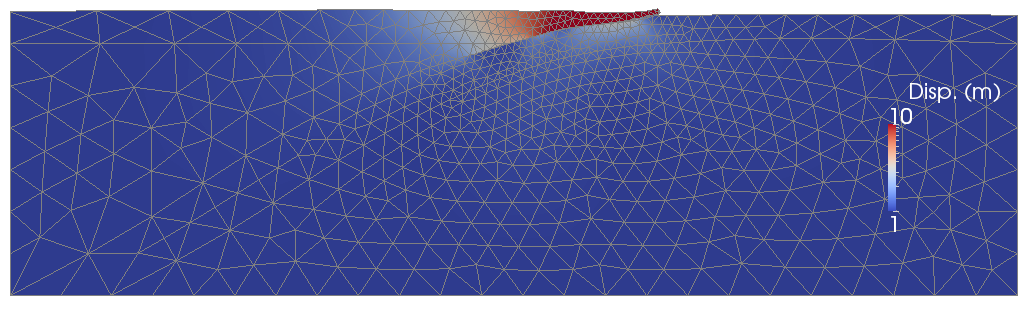
\includegraphics[width=4.5in]{examples/figs/subduction2d_step01_soln}
  \caption{Solution for Step 1. The colors indicate the magnitude of the displacement,
    and the deformation is exaggerated by a factor of 1000. }
  \label{fig:example:subduction:2d:step01}
\end{figure}


\subsubsection{Exercises}

% Algebraic multigrid preconditioner
% Adjust material properties (stiffer, softer, nearly incompressible)
% Pure shear instead of axial compression

\subsection{Step 2: Postseismic Relaxation}

\subsubsection{Exercises}

% Change slip on slab to slip on splay fault
% Slip on lower slab and splay fault
% Slip on slab and splay fault

\subsection{Step 3: Interseismic Deformation}

\subsubsection{Exercises}

\subsection{Step 4: Prescribed Earthquake Cycle}

\subsubsection{Exercises}

% Make lower slab + splay fault the primary fault surface and the
% upper slab (trench side of the splay fault) the secondary fault
% surface. Hint: You will need to create a nodesets in CUBIT that
% correspond to the primary and secondary fault surfaces.



\subsection{Step 5: Spontaneous Rupture Driven by Subducting Slab}

\subsubsection{Exercises}

\subsection{Step 6: Prescribed Slow-Slip Event}

\subsubsection{Exercises}

% Change spatial distribution and time history of slip.

\subsection{Step 7: Inversion of Slow-Slip using 3D Green's Functions}

\subsubsection{Exercises}

% Move slip to splay fault in step06 and redo inversion.
% Adjust noise level
% Invert for slip at each time step

\subsection{Step 8: Gravitational Body Forces}


% End of file
